\section{Consonants}

In this paragraph about consonants, I would like to begin with the definition of a consonant.

\newglossaryentry{cons}{name=C, description={Consonant}}

\textit{Consonant\index{consonant} (\gls{cons})} - a sound that is articulated with complete or particular closure of the vocal tract. 

Likewise vowels, consonants have three characteristics that determine their position in your articulation. These three parameters are:

\begin{itemize}
	\item{Place, where the consonant is pronounced in the mouth}
	\item{Manner, how the consonant is pronounced }
	\item{Sonority, whether you use your vocal cords or not}
\end{itemize}

\textbf{Place\index{consonant!place}} of the consonant can be quite different. Here are possible types: \textit{Bilabial, labiodental, dental, alveolar, postalveolar, palato-alveolar, retroflex, alveolo-palatal, palatal, labio-velar, velar}. There are more types, but they do not exist in Novoslovnica.

\textbf{Manner\index{consonant!manner}} is the way how you pronounce the sound. There are also different manners, that are used in Novoslovnica. They are: \textit{nasal, stop, affricate (sibilant), sibilant fricative, non-sibilant fricative, approximant, trill, lateral approximant}.

\textbf{Sonority\index{consonant!sonority}} is the boolean attribute of pronunciation. You can either use your voice \textit{with} the sound you pronounce or \textit{not}. Notice that vowels cannot be pronounced without the use of your voice. 

Combining these three parameters, we get the unique consonant that we want to pronounce. We cannot draw  a 3-dimensional table, because there are three parameters on input, so we will combine information into 2-dimensional space as in paragraph about vowels. So, look at the figure and see the different consonants that are used in Novoslovnica.

\begin{figure}[h]
	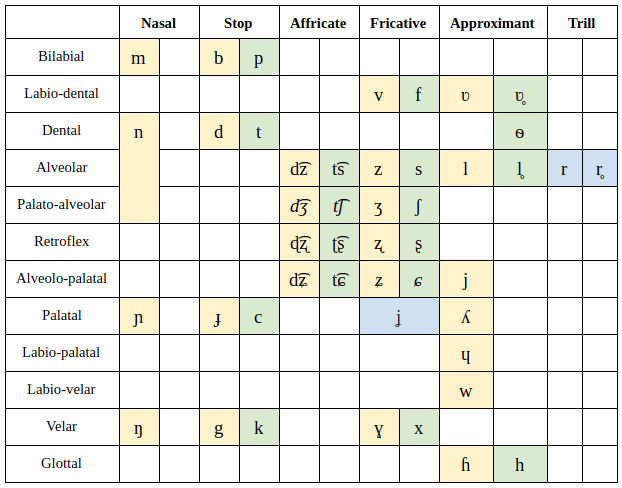
\includegraphics[width=\linewidth]{./sources/consonants.png}
	\caption{Consonant sounds in Novoslovnica}
	\label{fig:consonants}
\end{figure}

Different colors of the cells show the sonority of the consonant. Yellow color shows that the sound is voiced, while green ones are for voiceless sounds.

Blue cells in the table show that sounds in it can be used both in voiced and voiceless forms as allophones.

Novoslovnica has 51 consonants, 21 of them are voiceless and 30 are voiced.

However, not all of these consonants are language phonemes. So, let’s talk about the allophones among these sounds.

\begin{table}[h]
	\caption{Consonant allophones in Novoslivnica }
	\begin{tabular}{ll}
		Main consonant & Allophones \\
		\textipa{\t{\:d\textctz}} & \textipa{\t{\:dZ}} \\
		\textipa{\t{tC}}  & \textipa{\t{tS}} \\
		 \textipa{Z} & \textipa{\textctz}  \\
		  \textipa{S}  &  \textipa{C} \\
		  \textipa{l}   &  \textipa{(\r*l} \\
		   \textipa{r} (voiced)  &  \textipa{r} (voiceless) \\
		   \textipa{n} (alveolar) & \textipa{n} (palato-alveolar), \textipa{n} (dental) \\
		    \textipa{(\r*r} (voiced) & \textipa{(\r*r} (voiceless) \\
		    \textipa{v} & \textipa{V} \\
		    \textipa{f} & \textipa{\r*V} \\
		    \textipa{H} & \textipa{G} \\
		    \textipa{x} & \textipa{h} \\
	\end{tabular}
\end{table}

Likewise vowels, consonants can be compared with each other in terms of softness/hardness. The common rule is that every consonant has its soft or hard partner.

Exception: Three sounds are exceptions to this rule.
The sound \textipa{T} has no pair, because its pair ð has never been used in Slavic languages.
Also nasal velar consonant \textipa{N} has no soft pair.
And vice versa, the sound j is soft and has no hard pair. 

Remember this exception, let’s look at the table 1.7 to get acquainted with pairs of consonants.

\begin{longtable}{ll}
%	\caption{Softness in Novoslivnica}
		Hard consonant & Soft consonant \\
		\endhead 
		b & bj \\
		v & vj \\
		g & gj \\
		\textipa{H} & \textipa{Hj} \\
		d & \textipa{J} \\
		\textipa{\t{\:d\:z}} & \textipa{\t{\:d\textctz}} \\
		\textipa{\t{dz}} & \textipa{\t{dzj}} \\
		\textipa{\:z} & \textipa{Z}  \\
		z & zj \\
		k & kj \\
		l & \textipa{L} \\
		m & mj \\
		n & \textltailn \\ 
		p & pj \\
		r & rj \\
		\textipa{\r*r} & \textipa{\r*rj} \\
		s & sj \\
		t & \textipa{C} \\
		f & fj \\
		x & xj \\
		\textipa{\t{ts}} & \textipa{\t{tsj}} \\
		\textipa{\t{t\:s}}  & \textipa{\t{tC}} \\
		\textipa{\:s} & \textipa{S} \\
		w & \textvibyy \\
\end{longtable}

As you see, every consonant from table has its own soft pair. The soft consonant is usually written as a hard consonant with the sound j attached, but some of them are provided as unique sounds by IPA, because in some languages they can be phonemes. (footnote)


% любопытным следтвием наличия особых значков в IPA для мягких были попытки построения чисто фонетических алфавитов на основе только символов IPA, которые должны были использоваться в качестве букв. (дополнение можно внести в текст книги).